\section{Entwurf}

\subsection{Kommunikationseinheit} \label{commModule}

\subsubsection{init/0}

Beim Initialisieren einer Kommunikationseinheit wird ein Prozess gestartet, welcher beim \textit{towerCBC} registriert wird und bei der \textit{towerClock} eine neue Vektoruhr ID anfragt. Wie in Abb. \ref{fig:sequence_cbCast_init} zu sehen, wird der Aufruf an die \textit{towerClock} von dem Prozess gesendet, der auch beim \textit{towerCBC} registriert wird. Grund dafür ist, dass die \textit{towerClock} die Prozess ID des anfragenden Prozesses auf dessen Vektoruhr ID mappt. Würde der Prozess, welcher den \textit{cbCast} Prozess erzeugt diese Anfrage schicken, würde dieses Mapping eine falsche Prozess ID speichern.
\\Der Verbindungsaufbau oder auch Verbindungstest terminiert das Programm, wenn er fehlschlägt.
\\Nach Erzeugung des \textit{cbCast} Prozesses ist dieser sequenziell nicht mehr gebunden an den Prozess, der diesen erzeugt hat. Dementsprechend verlaufen die Aufrufe dieser beiden nebenläufig.

\begin{figure}[htbp]
\begin{center}
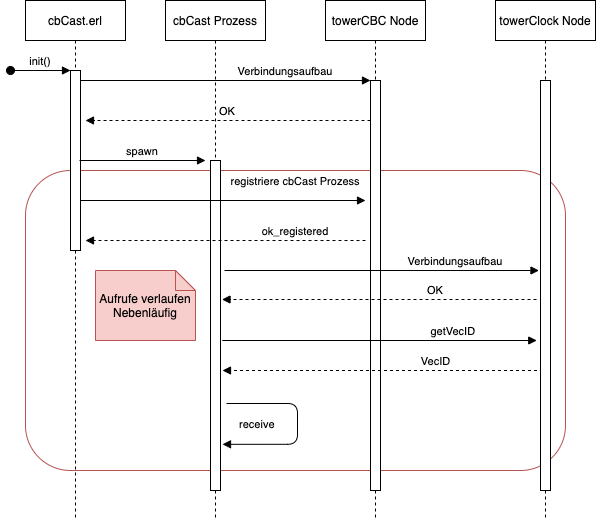
\includegraphics[scale=0.55]{Latex/Bilder/Sequenzdiagramm_cbCast.png}
\caption{\label{fig:sequence_cbCast_init} Sequenzdiagramm Initialisierung}
\end{center}
\end{figure}

Alternativ könnte sich der \textit{cbCast.erl} auch erst beim \textit{towerClock} die \textit{VektorID} holen und dann den \textit{cbCast} Prozess erzeugen. Durch den Ablauf in Abb. \ref{fig:sequence_cbCast_init} kann das Holen der \textit{VektorID} aber nebenläufig zur Registrierung beim \textit{towerCBC} passieren. Der ganze Vorgang ist somit schneller.

\subsubsection{stop/1} \label{commModule_stop}

Die Terminierung erfolgt auf zwei verschiedene Wege. Zuerst wird der Prozess gestoppt, das bedeutet, dass ein sogenannter \textit{Graceful Shutdown} durchgeführt wird. Hat dieser kein Erfolg, wird der Prozess durch einen \textit{Hard Shutdown} gekillt.\\
Als Parameter wird der zu terminierende Prozess übergeben.

\subsubsection{send/2} \label{commModule_send}

Beim Senden (siehe Abb. \ref{fig:sequence_cbCast_send}) wird eine Nachricht \textit{(Msg)} an den als Parameter übergebenen \textit{Kommunikationsprozess (cbCast Prozess)} geschickt. Dieser erhöht seine Vektoruhr vor dem Senden um 1 und verschickt die Nachricht an den \textit{Multicast}. Der \textit{Multicast} verteilt die Nachricht an alle Prozesse, inklusive dem Sender.\\
Die Vektoruhr der versendeten Nachricht hat zu der Vektoruhr der \textit{Kommunikationseinheit} eine Distanz von -1, wodurch diese Nachricht auslieferbar ist und direkt in die \textit{Delivery Queue} einsortiert werden kann.\\
Aufgrund des manuellen Modus des \textit{Multicasts} muss die Nachricht direkt in die \textit{Delivery Queue} einsortiert werden. Für einen sauberen Ablauf und zum Sicherstellen der kausalen Ordnung wäre es angenehmer die Nachricht nach dem Senden wieder zu empfangen und durch die \textit{Holdback Queue} laufen zu lassen, dies ist aber nicht möglich. Angenommen \textit{Kommunikationsprozess} N versendet eine Nachricht, welche nicht direkt in der \textit{Delivery Queue} gespeichert wird, dann wird vor dem Versenden die Vektoruhr um 1 erhöht. Beim Empfangen der Nachricht würde die Distanz der Vektoruhr der Nachricht und der Vektoruhr des \textit{Kommunikationsprozesses} eine Distanz von 0 haben (siehe Abb. \ref{fig:cbCast_scenario_1}). Um in die \textit{Delivery Queue} sortiert zu werden, muss diese Distanz -1 sein, was durch das weitere Erhöhen der Vektoruhr des Prozesses nicht mehr möglich ist (siehe Abb. \ref{fig:cbCast_scenario_2}).

\begin{figure}[htbp]
\begin{center}
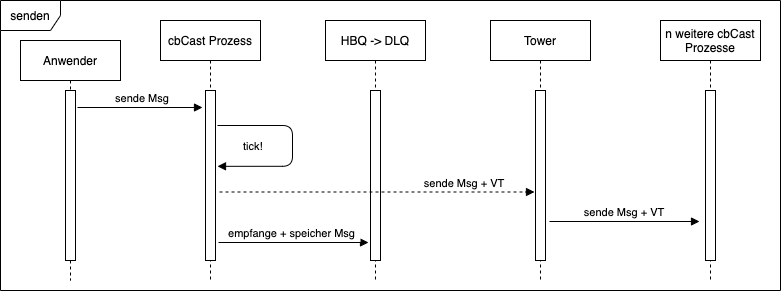
\includegraphics[scale=0.5]{Latex/Bilder/Sequenz_senden.png}
\caption{\label{fig:sequence_cbCast_send} Sequenzdiagramm Senden}
\end{center}
\end{figure}

\begin{figure}[htbp]
\begin{center}
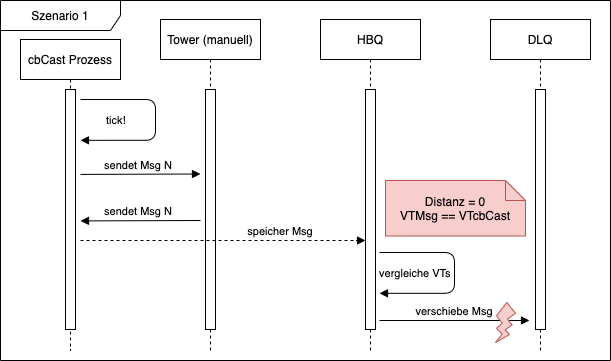
\includegraphics[scale=0.5]{Latex/Bilder/cbCast_szenario_1.png}
\caption{\label{fig:cbCast_scenario_1} Auslieferbarkeit im manuellen Modus - Szenario 1}
\end{center}
\end{figure}

\begin{figure}[htbp]
\begin{center}
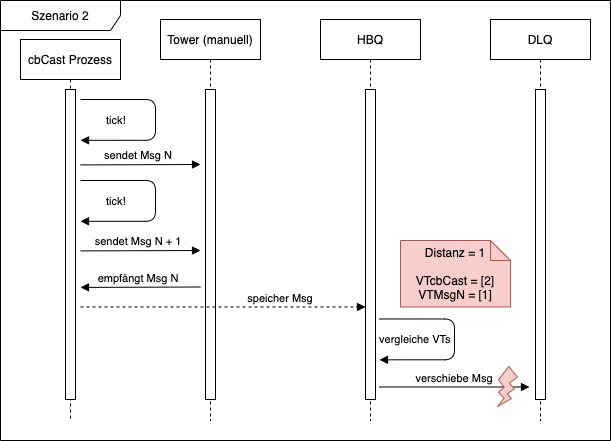
\includegraphics[scale=0.5]{Latex/Bilder/cbCast_szenario_2.png}
\caption{\label{fig:cbCast_scenario_2} Auslieferbarkeit im manuellen Modus - Szenario 2}
\end{center}
\end{figure}

\newpage

\subsubsection{read/1 \& received/1}

\begin{figure}[htbp]
\begin{center}
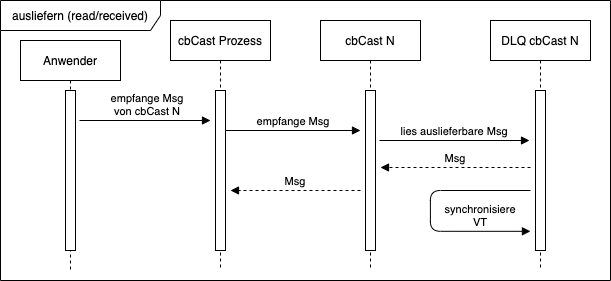
\includegraphics[scale=0.5]{Latex/Bilder/Sequenz_ausliefern.png}
\caption{\label{fig:sequence_cbCast_read_receive} Sequenzdiagramm Ausliefern}
\end{center}
\end{figure}

Das Ausliefern einer Nachrichten (siehe Abb. \ref{fig:sequence_cbCast_read_receive}) liest eine Nachricht aus der \textit{Delivery Queue} des \textit{Kommunikationsprozesses (cbCast N)}, welcher als Parameter übergeben wurde. Gelesen wird die der \textit{Delivery Queue} zuerst hinzugefügte Nachricht. Eine Nachricht kann nur einmal gelesen werden und wird dabei aus der Queue entfernt.\\
Für das Ausliefern gibt es eine Funktion welche blockierend und eine, welche nicht blockierend empfängt.

\paragraph{read/1 (nicht blockierend)}

Falls der angefragte Prozess keine auslieferbare Nachricht zur Verfügung hat, wird nichts empfangen und der anfragende Prozess läuft normal weiter.

\paragraph{receive/1 (blockierend)}

Falls der angefragte Prozess keine auslieferbare Nachricht zur Verfügung hat, wartet der anfragende Prozess so lange, bis eine auslieferbare Nachricht empfangen wird.\\

In beiden Funktionen synchronisiert der angefragte Prozess anschließend seine Vektoruhr mit der der ausgelieferten Nachricht, falls eine Nachricht verschickt wurde.

\subsubsection{$\{\langle PID \rangle,\{castMessage,\{\langle Message \rangle, \langle VT \rangle\}\}\}$}

Wenn der \textit{Multicast (Tower)} eine Nachricht verschickt, wird diese von der Schnittstelle $\{\langle PID \rangle,\{castMessage,\{\langle Message \rangle, \langle VT \rangle\}\}\}$ des \textit{Kommunikationsprozesses} empfangen (siehe Abb. \ref{fig:sequence_cbCast_cbcast}). Daraufhin wird die Nachricht in der \textit{Holdback Queue} des Prozesses gepusht. Aus in  Kapitel \ref{hbq_theory} genannten Gründen, werden neue Nachrichten immer am Anfang der Queue gespeichert. Wenn die empfangene Nachricht von dem Prozess stammt, der sie empfangen hat, wird sie nicht in der \textit{Holdback Queue} gespeichert, sondern verworfen. Das ist möglich durch das Speichern der Nachricht in der \textit{Delivery Queue} beim Versenden (siehe Kapitel \ref{commModule_send}).

\begin{figure}[htbp]
\begin{center}
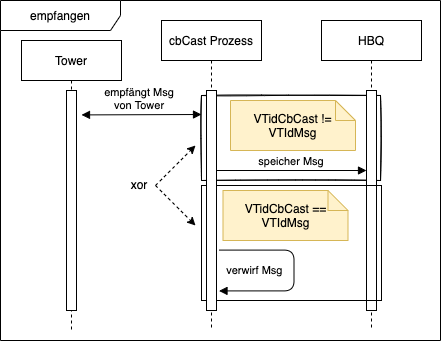
\includegraphics[scale=0.5]{Latex/Bilder/Sequenz_empfangen.png}
\caption{\label{fig:sequence_cbCast_cbcast} Sequenzdiagramm Empfangen}
\end{center}
\end{figure}

\paragraph{checkQueues/3} überprüft die \textit{Holdback Queue} auf auslieferbare Nachrichten. Ist eine Nachricht auslieferbar, wird sie an den Anfang der \textit{Delivery Queue} gepusht.\\
Diese Prüfung muss gemacht werden, wenn eine Nachricht in die \textit{Holdback Queue} hinzugefügt wird und sobald die Vektoruhr des \textit{Kommunikationsprozesses} verändert wird. Dies betrifft also die Schnittstellen \textbf{send/2}, \textbf{read/1}, \textbf{receive/1} und\\ $\{\langle PID \rangle,\{castMessage,\{\langle Message \rangle, \langle VT \rangle\}\}\}$ und wird am Ende der jeweiligen Schnittstelle aufgerufen.

\subsection{Vektoruhr-ADT} \label{vectorC_entwurf}

Die Datenstruktur der Vektoruhr besteht aus einem Tupel mit zwei Elementen. Das erste Element zeigt die Identität der Vektoruhr. Das zweite Element zeigt die eigentliche Vektoruhr, bestehend aus einer Liste aus natürlichen ganzen positiven Zahlen, inklusive der 0.\\
Die Zahlen in der Liste zeigen den Zeitstempel der verschiedenen \textit{Kommunikationsprozesse}. Die Identität ist der Index in der Liste, welcher den eigenen Zeitstempel zeigt.

\subsubsection{initVT/0}

Diese Schnittstelle initialisiert eine leere Vektoruhr. Um die richtige Identität zu kennen, wird diese bei der Vektoruhr Zentrale angefragt (siehe Kapitel \ref{tower} und Abb. \ref{fig:sequence_cbCast_init}). Die Identität ist gleichzeitig die Länge der initialen Liste. Alle Zustände sind bei Initialisierung 0. Eine leere Vektoruhr könnte also $\{1, [0]\}$ oder $\{5, [0,0,0,0,0]\}$ sein.

\subsubsection{myVTid/1}

MyVTid gibt die Identität der übergebenen Vektoruhr zurück. 

\subsubsection{myVTvc/1}

MyVTvc gibt die eigentliche Vektoruhr als Liste zurück.

\subsubsection{myCount/1}

MyCount gibt den eigenen Zeitstempel der im Parameter übergebenen Vektoruhr zurück. Dieser ergibt sich anhand der Identität und der eigentlichen Vektoruhr. $\{1, [5]\}$ hat den Zeitstempel 5 und $\{5, [1,1,4,2,7,3,3]\}$ hat den Zeitstempel 7.

\subsubsection{foCount/2}

Als Parameter werden eine Vektoruhr und ein Index übergeben. Zurückgegeben wird der Zeitstempel der übergebenen Vektoruhr am übergebenen Index. Der Index muss größer als 0 sein.

\subsubsection{isVT/1}

IsVT prüft ob die übergebene Vektoruhr syntaktisch korrekt ist.

\subsubsection{syncVT/2}

Diese Schnittstelle empfängt zwei Vektoruhren. Zuerst werden beide Vektoruhren auf die gleiche Länge mit 0en aufgefüllt. Anschließend werden die normalisierten Vektoren verglichen. Es wird eine neue Vektoruhr mit der Identität des zuerst übergebenen Vektors zurückgegeben. Diese repräsentiert das Maximum aus beiden übergebenen Vektoruhren. Aus $\{3, [1,4,3]\}$ und $\{4, [2,3,1,5]\}$ wird also $\{3, [2,4,3,5]\}$. 

\subsubsection{tickVT/1}

TickVT erhöht den eigenen Zeitstempel der übergebenen Vektoruhr um 1. Aus $\{2, [2,1]\}$ wird also $\{2, [2,2]\}$.

\subsubsection{compVT/2} \label{vectorC_comp}

CompVT vergleicht zwei übergebene Vektoruhren. Hierbei gibt es vier verschiedene\\ Rückgabewerte. Diese Rückgabewerte sind die Positionen die die beiden Vektoruhren zueinander haben (genauer beschrieben in Kapitel \ref{hbq_theory}).\\
Nach der Normalisierung der Vektoruhren werden die beiden Vektoren elementweise verglichen. Dabei wird ein Vergleichszustand zurückgegeben, der angibt, ob ein Vektorzeitstempel logisch vor, nach oder gleich der anderen ist. Der Vergleich erfolgt rekursiv, wobei die Vektoren jeweils um das erste Element verkürzt werden und das Ergebnis Schritt für Schritt aktualisiert wird.
\begin{itemize}
    \item \textit{After} sind zwei Vektoruhren (VT1 \textit{after} VT2), wenn der Vergleichzustand in einem Durchlauf ausschließlich logisch nach oder gleich ist.
    \item \textit{Before} wenn er ausschließlich logisch vor oder gleich ist.
    \item \textit{Equal} sind die Vektoren, wenn der Vergleichzustand ausschließlich logisch gleich ist.
    \item \textit{Concurrent} also nebenläufig sind zwei Vektoruhren zueinander, wenn der Vergleichszustand in einem Durchlauf von logisch vor zu logisch nach oder umgekehrt wechselt.
\end{itemize}

\subsubsection{aftereqVTJ/2} \label{aftereqvtj_entwurf}

Diese Schnittstelle vergleicht im Sinne des kausalen Multicast die zwei übergebenen Vektoruhren VT und VTR.
Dafür wird in beiden Vektoruhren zunächst das Element an der Stelle J entfernt, wobei J die Identität der Vektoruhr VTR darstellt.
Die beiden neuen Vektoruhren werden nun über \textit{compVT/2} (siehe Kapitel \ref{vectorC_comp}) miteinander verglichen. Wenn VT logisch nach oder gleich VTR ist, dann wird die Distanz zwischen den beiden entfernten Elementen zueinander zurückgegeben, also VT[J] - VTR[J].

\subsection{Ungeordneter Multicast}

\subsubsection{init/1} \label{towercbc_init_entwurf}

Bei der Initialisierung des \textit{Multicasts} (auch \textit{Tower}) gibt es aus Testzwecken zwei verschiedene Modi (siehe Abb. \ref{fig:sequence_tower_init}). Zum einen kann der \textit{Tower} im Modus \textit{auto} gestartet werden, hierbei ist nur die Schnittstelle $\{\langle PID\rangle,\{multicastB,\{\langle Message\rangle,\langle VT\rangle\}\}\}$ der drei \textit{Multicast}-Schnittstellen erreichbar. Nachrichten, welche vom \textit{Tower} empfangen werden, werden direkt an alle Teilnehmer versendet und nicht gespeichert.\\
Im Modus \textit{manu} sind die beiden Schnittstellen $\{\langle PID\rangle,\{multicastNB,\{\langle Message\rangle,\langle VT\rangle\}\}\}$ und $\{\langle PID\rangle,\{multicastM,\langle CommNR\rangle,\langle MessageNR\rangle\}\}$ verfügbar. Zusätzlich kann vom Anwender die Schnittstelle \textit{cbcast/2} (siehe Kapitel \ref{tower_cbcast}) aufgerufen werden. Im Gegensatz zum Modus \textit{auto} werden empfangene Nachrichten gespeichert und können mehrfach versendet werden.

\begin{figure}[htbp]
\begin{center}
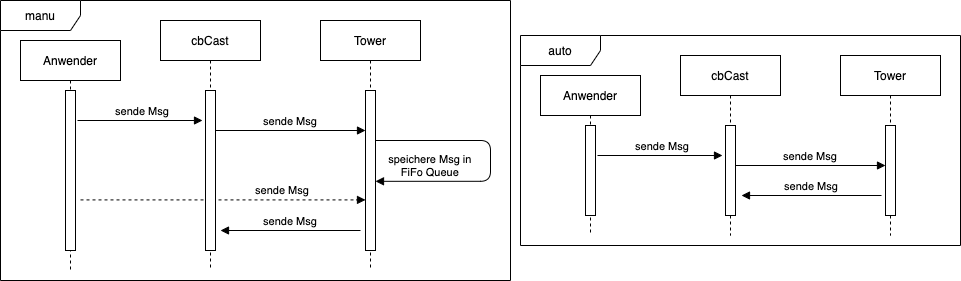
\includegraphics[scale=0.45]{Latex/Bilder/towerCBC_init.png}
\caption{\label{fig:sequence_tower_init} \textit{Tower}: Vgl. \textit{manu/auto}}
\end{center}
\end{figure}


\subsubsection{stop/1}

Die Schnittstelle \textit{stop} stoppt den entsprechend übergebenen \textit{Tower}. Wie auch bei der Kommunikationseinheit wird die Terminierung auf zwei verschiedenen Wegen durchgeführt (siehe Kapitel \ref{commModule_stop}).

\subsubsection{listall/0}

\textit{Listall} loggt alle, beim \textit{Tower} registrierten, \textit{Kommunikationsprozesse}. Hierbei wird lediglich die Prozess ID geloggt.

\subsubsection{cbcast/2} \label{tower_cbcast}

Diese Schnittstelle ermöglicht das manuelle Senden von bestimmten Nachrichten an bestimmte registrierte \textit{Multicast} Teilnehmer - in diesem Fall \textit{Kommunikationsprozesse}. Als Parameter werden zwei ganze natürliche Zahlen größer 0 erwartet. Sowohl die registrierten Teilnehmer als auch die empfangenen Nachrichten werden in zwei separaten FiFo Queues gespeichert. Die beiden übergebenen Zahlen sind die Indizes der beiden Listen. 

\subsubsection{$\{\langle PID \rangle,\{register,\langle RPID\rangle\}\}$}

Beim Senden an diese Schnittstelle wird die mitgesendete \textit{RPID} in einer Liste im \textit{Tower} gespeichert. Sobald die \textit{RPID} in dieser Liste enthalten ist, ist der Prozess hinter dieser ID beim \textit{Tower} registriert und kann  somit Nachrichten empfangen.

\subsubsection{$\{\langle PID\rangle,\{multicastB,\{\langle Message\rangle,\langle VT\rangle\}\}\}$}

\textit{MulticastB} steht in diesem Fall für ein blockierendes \textit{Multicasting}. Genutzt wird die Schnittstelle im Modus \textit{auto} des \textit{Towers}. Versendet ein Prozess eine Nachricht an \textit{multicastB}, wird die Nachricht an alle registrierten Teilnehmer versendet. Blockierend ist der Vorgang, da das Versenden nicht nebenläufig verläuft.

\subsubsection{$\{\langle PID\rangle,\{multicastNB,\{\langle Message\rangle,\langle VT\rangle\}\}\}$} 

\textit{MulticastNB} steht gegensätzlich zum \textit{multicastB} für nicht blockierend. Nachrichten werden von anderen Prozessen im Modus \textit{manu} des \textit{Towers} empfangen und nicht direkt weiterversendet. Stattdessen werden die empfangenen Nachrichten in einer FiFo Queue gespeichert, auf die der \textit{Tower} beim manuellen Senden über die Schnittstelle \textit{cbcast/2} (siehe Kapitel \ref{tower_cbcast}) zugreifen kann.

\subsubsection{$\{\langle PID\rangle,\{multicastM,\langle CommNR\rangle,\langle MessageNR\rangle\}\}$}

Die letzte Schnittstelle \textit{multicastM} versendet Nachrichten manuell. Während die anderen \textit{Multicast} Schnittstellen vom Anwender oder von anderen Prozessen aufgerufen werden, wird diese Schnittstelle vom \textit{Tower} selbst, bzw. über die Schnittstelle \textit{cbcast/2} (siehe Kapitel \ref{tower_cbcast}) aufgerufen.

\subsection{Vektoruhr Zentrale/Tower} \label{tower}

Die zentrale Vektoruhr (\textit{Tower}) verwaltet die Identitäten der jeweiligen \textit{Kommunikationsprozesse}. Die Identitäten sind eindeutige IDs aus positiven ganzen Zahlen, beginnend bei 1.
Aus Gründen der Erweiterbarkeit, wird die Identität zusammen mit der jeweiligen Prozess ID als Key Value Paar gespeichert.

\subsubsection{$\{getVecID,\langle PID\rangle\}$}

Beim Senden an diese Schnittstelle wird geprüft ob für den Prozess mit der ID \textit{PID} schon eine Identität angelegt wurde. Falls dies der Fall ist, wird die entsprechende Identität zurückgesendet. Wenn nicht, wird eine neue Identität erzeugt und zurückgeschickt. Ist N die zuletzt erzeugte Identität wird N + 1 die Nächste.

\subsubsection{init/0}

\textit{Init} erzeugt eine Vektoruhr Zentrale.

\subsubsection{stop/1}

Die Schnittstelle \textit{stop} stoppt die entsprechend übergebene Vektoruhr Zentrale. Wie auch bei der Kommunikationseinheit wird die Terminierung auf zwei verschiedenen Wegen durchgeführt (siehe Kapitel \ref{commModule_stop}).

\subsection{Generelle Designentscheidungen}

\subsubsection{Logging}

Pro Node wird eine generische .log Datei erstellt. Beispielweise gibt es für den Node \textit{'cbCast1@MacBook-Air-von-Kristoffer'} die Datei \textit{'cbCast1@MacBook-Air-von-Kristoffer'.log}. Dies bringt den Vorteil, dass die verschiedenen Kommunikationseinheiten - welche über die gleiche .beam Datei ausgeführt werden, aber auf verschiedenen Nodes laufen - separat voneinander geloggt werden.
\\Zum Debuggen war ein Gedanke, zusätzlich eine Logging Datei zu erstellen, in welcher alle Prozesse loggen. Hierdurch kann sequenziell nachverfolgt werden, ob die Reihenfolge der Aufrufe korrekt verläuft. Im Verlauf der Implementierung hat sich herausgestellt, dass diese Datei wenig Mehrwert bringt. Deswegen fehlt diese in der finalen Implementierung.